\subsubsection{Risultati}
\label{sct:meter_risultati}
\begin{figure}[p]
  \centering
  \begin{subfigure}[b]{.5\textheight}
    %% $ cd meter_data
    %% $ ./compact 2_4_*.dat
    %% $ ./printAll  2 4
    %% $ ./plot.sh 2 4
    %% $ cd ..
    %% $ cp meter_data/2_4_{sym,asymin}_all.{tex,pdf} ./
    \resizebox{\columnwidth}{!}{% GNUPLOT: LaTeX picture with Postscript
\begingroup
  \makeatletter
  \providecommand\color[2][]{%
    \GenericError{(gnuplot) \space\space\space\@spaces}{%
      Package color not loaded in conjunction with
      terminal option `colourtext'%
    }{See the gnuplot documentation for explanation.%
    }{Either use 'blacktext' in gnuplot or load the package
      color.sty in LaTeX.}%
    \renewcommand\color[2][]{}%
  }%
  \providecommand\includegraphics[2][]{%
    \GenericError{(gnuplot) \space\space\space\@spaces}{%
      Package graphicx or graphics not loaded%
    }{See the gnuplot documentation for explanation.%
    }{The gnuplot epslatex terminal needs graphicx.sty or graphics.sty.}%
    \renewcommand\includegraphics[2][]{}%
  }%
  \providecommand\rotatebox[2]{#2}%
  \@ifundefined{ifGPcolor}{%
    \newif\ifGPcolor
    \GPcolortrue
  }{}%
  \@ifundefined{ifGPblacktext}{%
    \newif\ifGPblacktext
    \GPblacktexttrue
  }{}%
  % define a \g@addto@macro without @ in the name:
  \let\gplgaddtomacro\g@addto@macro
  % define empty templates for all commands taking text:
  \gdef\gplbacktext{}%
  \gdef\gplfronttext{}%
  \makeatother
  \ifGPblacktext
    % no textcolor at all
    \def\colorrgb#1{}%
    \def\colorgray#1{}%
  \else
    % gray or color?
    \ifGPcolor
      \def\colorrgb#1{\color[rgb]{#1}}%
      \def\colorgray#1{\color[gray]{#1}}%
      \expandafter\def\csname LTw\endcsname{\color{white}}%
      \expandafter\def\csname LTb\endcsname{\color{black}}%
      \expandafter\def\csname LTa\endcsname{\color{black}}%
      \expandafter\def\csname LT0\endcsname{\color[rgb]{1,0,0}}%
      \expandafter\def\csname LT1\endcsname{\color[rgb]{0,1,0}}%
      \expandafter\def\csname LT2\endcsname{\color[rgb]{0,0,1}}%
      \expandafter\def\csname LT3\endcsname{\color[rgb]{1,0,1}}%
      \expandafter\def\csname LT4\endcsname{\color[rgb]{0,1,1}}%
      \expandafter\def\csname LT5\endcsname{\color[rgb]{1,1,0}}%
      \expandafter\def\csname LT6\endcsname{\color[rgb]{0,0,0}}%
      \expandafter\def\csname LT7\endcsname{\color[rgb]{1,0.3,0}}%
      \expandafter\def\csname LT8\endcsname{\color[rgb]{0.5,0.5,0.5}}%
    \else
      % gray
      \def\colorrgb#1{\color{black}}%
      \def\colorgray#1{\color[gray]{#1}}%
      \expandafter\def\csname LTw\endcsname{\color{white}}%
      \expandafter\def\csname LTb\endcsname{\color{black}}%
      \expandafter\def\csname LTa\endcsname{\color{black}}%
      \expandafter\def\csname LT0\endcsname{\color{black}}%
      \expandafter\def\csname LT1\endcsname{\color{black}}%
      \expandafter\def\csname LT2\endcsname{\color{black}}%
      \expandafter\def\csname LT3\endcsname{\color{black}}%
      \expandafter\def\csname LT4\endcsname{\color{black}}%
      \expandafter\def\csname LT5\endcsname{\color{black}}%
      \expandafter\def\csname LT6\endcsname{\color{black}}%
      \expandafter\def\csname LT7\endcsname{\color{black}}%
      \expandafter\def\csname LT8\endcsname{\color{black}}%
    \fi
  \fi
  \setlength{\unitlength}{0.0500bp}%
  \begin{picture}(7200.00,5040.00)%
    \gplgaddtomacro\gplbacktext{%
      \csname LTb\endcsname%
      \put(946,704){\makebox(0,0)[r]{\strut{} 0}}%
      \put(946,1128){\makebox(0,0)[r]{\strut{} 50}}%
      \put(946,1553){\makebox(0,0)[r]{\strut{} 100}}%
      \put(946,1977){\makebox(0,0)[r]{\strut{} 150}}%
      \put(946,2402){\makebox(0,0)[r]{\strut{} 200}}%
      \put(946,2826){\makebox(0,0)[r]{\strut{} 250}}%
      \put(946,3251){\makebox(0,0)[r]{\strut{} 300}}%
      \put(946,3675){\makebox(0,0)[r]{\strut{} 350}}%
      \put(2223,484){\makebox(0,0){\strut{}1}}%
      \put(3369,484){\makebox(0,0){\strut{}8}}%
      \put(4514,484){\makebox(0,0){\strut{}14}}%
      \put(5791,704){\makebox(0,0)[l]{\strut{} 0}}%
      \put(5791,1071){\makebox(0,0)[l]{\strut{} 0.05}}%
      \put(5791,1438){\makebox(0,0)[l]{\strut{} 0.1}}%
      \put(5791,1805){\makebox(0,0)[l]{\strut{} 0.15}}%
      \put(5791,2172){\makebox(0,0)[l]{\strut{} 0.2}}%
      \put(5791,2539){\makebox(0,0)[l]{\strut{} 0.25}}%
      \put(5791,2906){\makebox(0,0)[l]{\strut{} 0.3}}%
      \put(5791,3273){\makebox(0,0)[l]{\strut{} 0.35}}%
      \put(5791,3640){\makebox(0,0)[l]{\strut{} 0.4}}%
      \put(176,2189){\rotatebox{-270}{\makebox(0,0){\strut{}$\mathrm{L}_{\mathrm{com}} \; (\,\tau\,)$}}}%
      \put(6692,2189){\rotatebox{-270}{\makebox(0,0){\strut{}$\mathrm{L}_{\mathrm{com}} \; (\,\mu\mathrm{sec}\,)$}}}%
      \put(3368,154){\makebox(0,0){\strut{}number of hops}}%
    }%
    \gplgaddtomacro\gplfronttext{%
      \csname LTb\endcsname%
      \put(4804,4867){\makebox(0,0)[r]{\strut{}\texttt{ch\_sym\_udn}}}%
      \csname LTb\endcsname%
      \put(4804,4647){\makebox(0,0)[r]{\strut{}\texttt{ch\_sym\_sm\_rdyack\_no}}}%
      \csname LTb\endcsname%
      \put(4804,4427){\makebox(0,0)[r]{\strut{}\texttt{ch\_sym\_sm\_rdyack}}}%
      \csname LTb\endcsname%
      \put(4804,4207){\makebox(0,0)[r]{\strut{}\texttt{ch\_sym\_sm\_nullack}}}%
    }%
    \gplbacktext
    \put(0,0){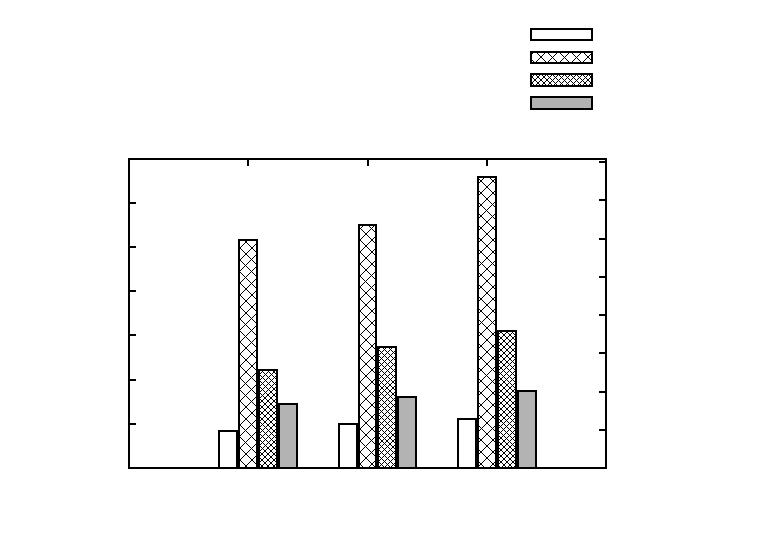
\includegraphics{2_5_sym_all_bw}}%
    \gplfronttext
  \end{picture}%
\endgroup
}
    \caption{Latenza di comunicazione misurata delle implementazioni del canale simmetrico}
    \label{fig:meter_ch_sym_2_4}
  \end{subfigure}
  \\
  \vspace{1cm}
  \begin{subfigure}[b]{.5\textheight}
    \resizebox{\columnwidth}{!}{% GNUPLOT: LaTeX picture with Postscript
\begingroup
  \makeatletter
  \providecommand\color[2][]{%
    \GenericError{(gnuplot) \space\space\space\@spaces}{%
      Package color not loaded in conjunction with
      terminal option `colourtext'%
    }{See the gnuplot documentation for explanation.%
    }{Either use 'blacktext' in gnuplot or load the package
      color.sty in LaTeX.}%
    \renewcommand\color[2][]{}%
  }%
  \providecommand\includegraphics[2][]{%
    \GenericError{(gnuplot) \space\space\space\@spaces}{%
      Package graphicx or graphics not loaded%
    }{See the gnuplot documentation for explanation.%
    }{The gnuplot epslatex terminal needs graphicx.sty or graphics.sty.}%
    \renewcommand\includegraphics[2][]{}%
  }%
  \providecommand\rotatebox[2]{#2}%
  \@ifundefined{ifGPcolor}{%
    \newif\ifGPcolor
    \GPcolortrue
  }{}%
  \@ifundefined{ifGPblacktext}{%
    \newif\ifGPblacktext
    \GPblacktexttrue
  }{}%
  % define a \g@addto@macro without @ in the name:
  \let\gplgaddtomacro\g@addto@macro
  % define empty templates for all commands taking text:
  \gdef\gplbacktext{}%
  \gdef\gplfronttext{}%
  \makeatother
  \ifGPblacktext
    % no textcolor at all
    \def\colorrgb#1{}%
    \def\colorgray#1{}%
  \else
    % gray or color?
    \ifGPcolor
      \def\colorrgb#1{\color[rgb]{#1}}%
      \def\colorgray#1{\color[gray]{#1}}%
      \expandafter\def\csname LTw\endcsname{\color{white}}%
      \expandafter\def\csname LTb\endcsname{\color{black}}%
      \expandafter\def\csname LTa\endcsname{\color{black}}%
      \expandafter\def\csname LT0\endcsname{\color[rgb]{1,0,0}}%
      \expandafter\def\csname LT1\endcsname{\color[rgb]{0,1,0}}%
      \expandafter\def\csname LT2\endcsname{\color[rgb]{0,0,1}}%
      \expandafter\def\csname LT3\endcsname{\color[rgb]{1,0,1}}%
      \expandafter\def\csname LT4\endcsname{\color[rgb]{0,1,1}}%
      \expandafter\def\csname LT5\endcsname{\color[rgb]{1,1,0}}%
      \expandafter\def\csname LT6\endcsname{\color[rgb]{0,0,0}}%
      \expandafter\def\csname LT7\endcsname{\color[rgb]{1,0.3,0}}%
      \expandafter\def\csname LT8\endcsname{\color[rgb]{0.5,0.5,0.5}}%
    \else
      % gray
      \def\colorrgb#1{\color{black}}%
      \def\colorgray#1{\color[gray]{#1}}%
      \expandafter\def\csname LTw\endcsname{\color{white}}%
      \expandafter\def\csname LTb\endcsname{\color{black}}%
      \expandafter\def\csname LTa\endcsname{\color{black}}%
      \expandafter\def\csname LT0\endcsname{\color{black}}%
      \expandafter\def\csname LT1\endcsname{\color{black}}%
      \expandafter\def\csname LT2\endcsname{\color{black}}%
      \expandafter\def\csname LT3\endcsname{\color{black}}%
      \expandafter\def\csname LT4\endcsname{\color{black}}%
      \expandafter\def\csname LT5\endcsname{\color{black}}%
      \expandafter\def\csname LT6\endcsname{\color{black}}%
      \expandafter\def\csname LT7\endcsname{\color{black}}%
      \expandafter\def\csname LT8\endcsname{\color{black}}%
    \fi
  \fi
  \setlength{\unitlength}{0.0500bp}%
  \begin{picture}(7200.00,5040.00)%
    \gplgaddtomacro\gplbacktext{%
      \csname LTb\endcsname%
      \put(946,704){\makebox(0,0)[r]{\strut{} 0}}%
      \put(946,1059){\makebox(0,0)[r]{\strut{} 50}}%
      \put(946,1413){\makebox(0,0)[r]{\strut{} 100}}%
      \put(946,1768){\makebox(0,0)[r]{\strut{} 150}}%
      \put(946,2122){\makebox(0,0)[r]{\strut{} 200}}%
      \put(946,2477){\makebox(0,0)[r]{\strut{} 250}}%
      \put(946,2831){\makebox(0,0)[r]{\strut{} 300}}%
      \put(946,3186){\makebox(0,0)[r]{\strut{} 350}}%
      \put(946,3540){\makebox(0,0)[r]{\strut{} 400}}%
      \put(946,3895){\makebox(0,0)[r]{\strut{} 450}}%
      \put(2256,484){\makebox(0,0){\strut{}1}}%
      \put(3435,484){\makebox(0,0){\strut{}8}}%
      \put(4613,484){\makebox(0,0){\strut{}14}}%
      \put(5923,704){\makebox(0,0)[l]{\strut{} 0}}%
      \put(5923,1317){\makebox(0,0)[l]{\strut{} 0.1}}%
      \put(5923,1930){\makebox(0,0)[l]{\strut{} 0.2}}%
      \put(5923,2543){\makebox(0,0)[l]{\strut{} 0.3}}%
      \put(5923,3156){\makebox(0,0)[l]{\strut{} 0.4}}%
      \put(5923,3769){\makebox(0,0)[l]{\strut{} 0.5}}%
      \put(176,2299){\rotatebox{-270}{\makebox(0,0){\strut{}$\mathrm{L}_{\mathrm{com}} \; (\,\tau\,)$}}}%
      \put(6692,2299){\rotatebox{-270}{\makebox(0,0){\strut{}$\mathrm{L}_{\mathrm{com}} \; (\,\mu\mathrm{sec}\,)$}}}%
      \put(3434,154){\makebox(0,0){\strut{}number of hops}}%
    }%
    \gplgaddtomacro\gplfronttext{%
      \csname LTb\endcsname%
      \put(4936,4867){\makebox(0,0)[r]{\strut{}\texttt{ch\_asymin\_udn}}}%
      \csname LTb\endcsname%
      \put(4936,4647){\makebox(0,0)[r]{\strut{}\texttt{ch\_asymin\_sm\_all}}}%
      \csname LTb\endcsname%
      \put(4936,4427){\makebox(0,0)[r]{\strut{}\texttt{ch\_asymin\_sm}}}%
    }%
    \gplbacktext
    \put(0,0){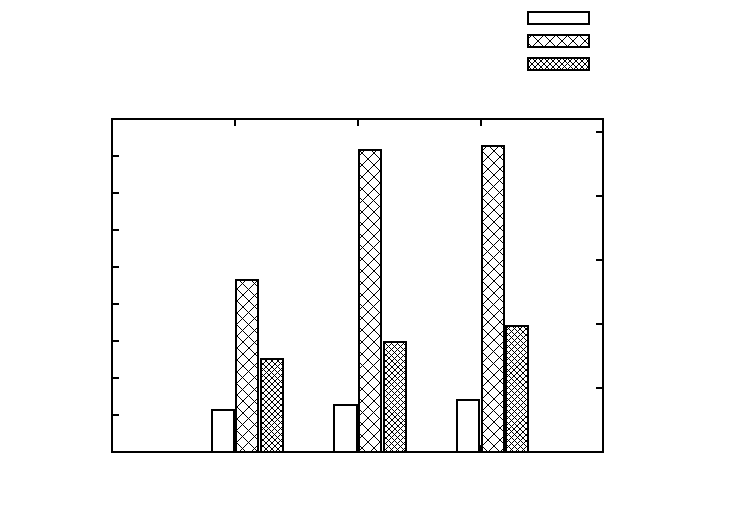
\includegraphics{2_5_asymin_all_bw}}%
    \gplfronttext
  \end{picture}%
\endgroup
}
    \caption{Latenza di comunicazione misurata delle implementazioni del canale asimmetrico in ingresso}
    \label{fig:meter_ch_asymin_2_4}
  \end{subfigure}
  \caption[Latenza di comunicazione dei canali]{Rappresentazione grafica dei risultati delle misurazioni della latenza di comunicazione dei canali. Il programma di misurazione \`e stato eseguito con un numero $m = 10^5$ di scambi e un numero $n = 10$ di iterazioni.}
  \label{fig:meter_type2_nscamb4}
\end{figure}

\begin{table}[!b]
  \centering
  \begin{subtable}[b]{\textwidth}
    \centering
    \begin{tabular}{|l|r|r|r|r|r|}
      \hline
      \multirow{3}{*}{\emph{Implementazione}} &
      \multirow{3}{4ex}{\emph{\# Hops}} &
      \multicolumn{4}{|c|}{$\inLcom$} \\
      \cline{3-6}
      & & \multicolumn{2}{|c|}{\emph{Avg}} &
      \multirow{2}{*}{\emph{Std Dev}} &
      \multirow{2}{*}{\emph{Max} $(\,\tau\,)$} \\
      \cline{3-4}
      & & $\tau$ & $\mu\mathrm{sec}$ & & \\
      \hline
      %% \multirow{3}{18ex}{\texttt{ch\_sym\_udn}} 
      %% & 1 & 42.066550 & 0.048655 & 0.097822 & 42.262000 \\
      %% & 8 & 49.561120 & 0.057323 & 0.104196 & 49.769500 \\
      %% & 14 & 55.722760 & 0.064450 & 0.107943 & 55.792050 \\
      %% \hline
      %% \multirow{3}{18ex}{\texttt{ch\_sym\_sm\_rdyack\_no}} 
      %% & 1 & 257.800490 & 0.298178 & 0.008955 & 257.815900 \\
      %% & 8 & 275.320380 & 0.318442 & 0.006685 & 275.327650 \\
      %% & 14 & 329.332180 & 0.380914 & 0.018220 & 329.363400 \\
      %% \hline
      %% \multirow{3}{18ex}{\texttt{ch\_sym\_rdyack\_sm}}
      %% & 1 & 111.482450 & 0.128943 & 0.187050 & 111.653200 \\
      %% & 8 & 137.378440 & 0.158895 & 0.016294 & 137.395550 \\
      %% & 14 & 155.377520 & 0.179713 & 0.013281 & 155.393950 \\
      %% \hline
      %% \multirow{3}{18ex}{\texttt{ch\_sym\_sm\_nullack}}
      %% & 1 & 72.359500 & 0.083692 & 0.219423 & 72.549500 \\ 
      %% & 8 & 80.700840 & 0.093340 & 0.124463 & 80.827350 \\ 
      %% & 14 & 86.759230 & 0.100347 & 0.118203 & 86.826250 \\
      \multirow{3}{*}{\texttt{ch\_sym\_udn}} 
      & 1 & 42.067 & 0.04866 & 0.09782 & 42.262 \\
      & 8 & 49.561 & 0.05732 & 0.10419 & 49.770 \\
      & 14 & 55.723 & 0.06445 & 0.10794 & 55.792 \\
      \hline
      \multirow{3}{*}{\texttt{ch\_sym\_sm\_rdyack\_no}} 
      & 1 & 257.800 & 0.29818 & 0.00896 & 257.816 \\
      & 8 & 275.320 & 0.31844 & 0.00669 & 275.328 \\
      & 14 & 329.332 & 0.38091 & 0.01822 & 329.363 \\
      \hline
      \multirow{3}{*}{\texttt{ch\_sym\_rdyack\_sm}}
      & 1 & 111.482 & 0.12894 & 0.18701 & 111.653 \\
      & 8 & 137.378 & 0.15890 & 0.01633 & 137.396 \\
      & 14 & 155.378 & 0.17971 & 0.01328 & 155.394 \\
      \hline
      \multirow{3}{*}{\texttt{ch\_sym\_sm\_nullack}}
      & 1 & 72.360 & 0.08369 & 0.21942 & 72.550 \\ 
      & 8 & 80.701 & 0.09334 & 0.12446 & 80.827 \\ 
      & 14 & 86.759 & 0.10034 & 0.11820 & 86.826 \\
      \hline
    \end{tabular}
    \caption[Latenza dei canali di comunicazione simmetrici]{Misurazione della latenza di comunicazione simmetrica delle diverse implementazioni.}
  \end{subtable}

  %%%%%%%%%%%%%%%%%%%%%%%%%%%%%%%%%%%%%%%%%%%%%%%%%%%%%%%%%%%%%%%%%%%%%%%%%%%%%%%%
  \vspace{4ex}
  %%%%%%%%%%%%%%%%%%%%%%%%%%%%%%%%%%%%%%%%%%%%%%%%%%%%%%%%%%%%%%%%%%%%%%%%%%%%%%%%

  \begin{subtable}[b]{\textwidth}
    \centering
    \begin{tabular}{|l|r|r|r|r|r|}
      \hline
      \multirow{3}{*}{\emph{Implementazione}} &
      \multirow{3}{4ex}{\emph{\# Hops}} &
      \multicolumn{4}{|c|}{$\inLcom$} \\
      \cline{3-6}
      & & \multicolumn{2}{|c|}{\emph{Avg}} &
      \multirow{2}{*}{\emph{Std Dev}} &
      \multirow{2}{*}{\emph{Max} $(\,\tau\,)$} \\
      \cline{3-4}
      & & $\tau$ & $\mu\mathrm{sec}$ & & \\
      \hline
      %% \multirow{3}{*}{\texttt{ch\_asymin\_udn}}
      %% & 1 & 56.025529 & 0.064800 & 0.000941 & 56.026905 \\
      %% & 8 & 63.525349 & 0.073475 & 0.000979 & 63.526575 \\
      %% & 14 & 69.527121 & 0.080416 & 0.001011 & 69.528720 \\
      %% \hline
      %% \multirow{3}{*}{\texttt{ch\_asymin\_sm\_all}}
      %% & 1 & 230.570268 & 0.266683 & 0.028743 & 230.643940 \\
      %% & 8 & 408.779285 & 0.472804 & 0.047859 & 408.846645 \\
      %% & 14 & 414.374837 & 0.479276 & 0.025326 & 414.417200 \\
      %% \hline
      %% \multirow{3}{*}{\texttt{ch\_asymin\_sm}}
      %% & 1 & 125.039207 & 0.144623 & 0.001632 & 125.041220 \\
      %% & 8 & 149.041103 & 0.172384 & 0.001936 & 149.045050 \\
      %% & 14 & 170.037299 & 0.196669 & 0.002036 & 170.040285 \\
      \multirow{3}{*}{\texttt{ch\_asymin\_udn}}
      & 1 & 56.0255 & 0.06480 & 0.00094 & 56.027 \\
      & 8 & 63.525 & 0.07348 & 0.00098 & 63.527 \\
      & 14 & 69.527 & 0.08042 & 0.00101 & 69.529 \\
      \hline
      \multirow{3}{*}{\texttt{ch\_asymin\_sm\_all}}
      & 1 & 230.570 & 0.26668 & 0.02874 & 230.644 \\
      & 8 & 408.779 & 0.47280 & 0.04786 & 408.847 \\
      & 14 & 414.375 & 0.47928 & 0.02533 & 414.417 \\
      \hline
      \multirow{3}{*}{\texttt{ch\_asymin\_sm}}
      & 1 & 125.039 & 0.14462 & 0.00163 & 125.041 \\
      & 8 & 149.041 & 0.17238 & 0.00194 & 149.045 \\
      & 14 & 170.037 & 0.19667 & 0.00204 & 170.040 \\
      \hline
    \end{tabular}
    \caption{Misurazione della latenza di comunicazione asimmetrica in ingresso delle diverse implementazioni.}
  \end{subtable}

  \caption[Latenza dei canali di comunicazione asimmetrici]{Misure della latenza di comunicazione rilevate iterando 10 volte il programma ``ping-pong'' con $m = 10^5$ scambi }
  \label{tab:meter}
\end{table}

I risultati proposti in tabella~\ref{tab:meter} e graficamente in figura~\ref{fig:meter_type2_nscamb4}, sono relativi a 10 iterazioni del programma di misurazione con $m = 10^5$ scambi di messaggi tra i due processi.

I risultati ottenuti verificano i ragionamenti descritti nelle Sezioni \ref{sct:specifica_sm}, \ref{sct:specifica_udn} che hanno guidato la realizzazione delle diverse implementazioni. La prima considerazione riguarda il confronto tra l'uso della UDN e della memoria condivisa: in entrambe le forme di comunicazione l'implementazione di UDN ha latenza inferiore a quella dell'implementazione con memoria condivisa pi\`u veloce. Raffiniamo questa osservazione valutando quale sia la migliore implementazione su memoria condivisa e quindi confrontiamola con l'implementazione UDN. La migliore implementazione su SM non \`e necessariamente quella pi\`u veloce: sebbene il protocollo Null-Ack fornisca la minor latenza, la sua implementazione fa uso di un valore particolare dei messaggi e pertanto \`e meno generica delle altre implementazioni. Ad esempio se si richiedesse una implementazione di canali di tipo generico, l'applicazione di questo protocollo potrebbe essere problematica. L'implementazione Null-Ack \`e utile per conoscere quale \`e la degradazione introdotta dalla barriera di memoria, necessaria nel protocollo Rdy-Ack, e quindi quale \`e il vero overhead della nostra implementazione lock-free dei canali. 

Passiamo a valutare la differenza tra le due implementazioni su SM che usano il protocollo Rdy-Ack e che differiscono per la gestione della gerarchia cache. Una gestione esplicita dell'allocazione in cache, che massimizzi la localit\`a dei dati, dimezza la latenza di comunicazione rispetto alla gestione predefinita dell'allocazione. Questo \`e un risultato generale, l'impostazione del PE consumatore come Home per il dato acceduto in computazioni \emph{consumatore~-~produttore} risulta determinante per ottimizzare le prestazioni; considerazioni simili sono state valutate in contesti differenti \cite{buono2013parallel}. Consideriamo quindi la \verb+ch_sym_sm_rdyack+ come implementazione candidata su memoria condivisa, che usa il protocollo Rdy-Ack. Osserviamo che il rapporto tra la latenza di questa soluzione e quella con il protocollo Null-Ack (sempre su SM) \`e di 1.68. Dato che le due implementazioni eseguono istruzioni simili, con la solo differenza della barriera di memoria, \`e ragionevole valutare la causa di questo aumento della latenza come l'esecuzione della memory fence.\\
Si osserva inoltre che l'implementazione Rdy-Ack \`e leggermente pi\`u sensibile alla variazione di distanza dei due processi, rispetto alla Null-Ack; quest'ultima ha un aumento della latenza pari a tanti cicli di clock quanto \`e l'aumento della distanza. Si nota che in questo aspetto la Null-Ack si comporta come la UDN. 
%%La seconda osservazione sulle implementazioni SM riguarda la gestione esplicita della gerarchia cache al fine di massimizzare la localit\`a dei dati: questa possibilit\`a risulta essere fondamentale per le prestazioni su memoria condivisa. L'uso della gestione predefinita \`e due volte pi\`u lento della versione con il descrittore di canale partizionato e homed nelle caches consumatori. \\
%%Si considera \verb+ch_sym_sm_rdyack+ l'implementazione migliore su SM. 

Si considera infine il rapporto tra la soluzione su SM e quella su UDN. Il vantaggio di uso dell'implementazione UDN rispetto a quella SM \`e significativo: mediamente la latenza UDN \`e inferiore pi\`u della met\`a (1/2.737) di quella SM. 

Il confronto dei canali asimmetrici con un singolo mittente ha risultato simile al confronto precedente. In questo caso il rapporto medio tra la latenze UDN e quella SM, 1/2.341, \`e leggermente maggiore. \`E significativo anche il confronto tra questi canali e i corrispondenti simmetrici, in quanto, nel programma di misurazione, i canali asimmetrici sono utilizzati per realizzare forme di comunicazione simmetrica. In entrambi i casi si ha un aumento della latenza di circa 10 cicli di clock. Ci\`o pu\`o essere spiegato dalle specifiche implementazioni parallele: con l'uso della UDN il mittente invia due parole, anzich\`e una del caso simmetrico; con l'uso della SM abbiamo l'uso di altre variabili, ad esempio per garantire la fairness, rispetto al caso simmetrico. \\
Si osserva infine che esiste una differenza sostanziale tra l'uso del canale asimmetrico su SM con un singolo mittente rispetto a quello con tutti i mittenti, ma uno solo attivo. La latenza nel secondo caso \`e mediamente il doppio di quella con un singolo mittente, ne segue un divario ancora pi\`u ampio con la latenza del canale su UDN.\\



%% media dei rapporti tra rdyack e nullack 1.678
%% media dei rapporti tra rdyack_no e rdy ack 2.145
%% media dei rapporti tra udn e rdyack 2.737
%% media dei rapporti tra asym_udn e asym_sm 2.341
%% media dei rapporti tra asym_udn e asym_sm_all 5.503





%% \begin{figure}[!h]
%%   \centering
%%   \resizebox{\columnwidth}{!}{% GNUPLOT: LaTeX picture with Postscript
\begingroup
  \makeatletter
  \providecommand\color[2][]{%
    \GenericError{(gnuplot) \space\space\space\@spaces}{%
      Package color not loaded in conjunction with
      terminal option `colourtext'%
    }{See the gnuplot documentation for explanation.%
    }{Either use 'blacktext' in gnuplot or load the package
      color.sty in LaTeX.}%
    \renewcommand\color[2][]{}%
  }%
  \providecommand\includegraphics[2][]{%
    \GenericError{(gnuplot) \space\space\space\@spaces}{%
      Package graphicx or graphics not loaded%
    }{See the gnuplot documentation for explanation.%
    }{The gnuplot epslatex terminal needs graphicx.sty or graphics.sty.}%
    \renewcommand\includegraphics[2][]{}%
  }%
  \providecommand\rotatebox[2]{#2}%
  \@ifundefined{ifGPcolor}{%
    \newif\ifGPcolor
    \GPcolortrue
  }{}%
  \@ifundefined{ifGPblacktext}{%
    \newif\ifGPblacktext
    \GPblacktexttrue
  }{}%
  % define a \g@addto@macro without @ in the name:
  \let\gplgaddtomacro\g@addto@macro
  % define empty templates for all commands taking text:
  \gdef\gplbacktext{}%
  \gdef\gplfronttext{}%
  \makeatother
  \ifGPblacktext
    % no textcolor at all
    \def\colorrgb#1{}%
    \def\colorgray#1{}%
  \else
    % gray or color?
    \ifGPcolor
      \def\colorrgb#1{\color[rgb]{#1}}%
      \def\colorgray#1{\color[gray]{#1}}%
      \expandafter\def\csname LTw\endcsname{\color{white}}%
      \expandafter\def\csname LTb\endcsname{\color{black}}%
      \expandafter\def\csname LTa\endcsname{\color{black}}%
      \expandafter\def\csname LT0\endcsname{\color[rgb]{1,0,0}}%
      \expandafter\def\csname LT1\endcsname{\color[rgb]{0,1,0}}%
      \expandafter\def\csname LT2\endcsname{\color[rgb]{0,0,1}}%
      \expandafter\def\csname LT3\endcsname{\color[rgb]{1,0,1}}%
      \expandafter\def\csname LT4\endcsname{\color[rgb]{0,1,1}}%
      \expandafter\def\csname LT5\endcsname{\color[rgb]{1,1,0}}%
      \expandafter\def\csname LT6\endcsname{\color[rgb]{0,0,0}}%
      \expandafter\def\csname LT7\endcsname{\color[rgb]{1,0.3,0}}%
      \expandafter\def\csname LT8\endcsname{\color[rgb]{0.5,0.5,0.5}}%
    \else
      % gray
      \def\colorrgb#1{\color{black}}%
      \def\colorgray#1{\color[gray]{#1}}%
      \expandafter\def\csname LTw\endcsname{\color{white}}%
      \expandafter\def\csname LTb\endcsname{\color{black}}%
      \expandafter\def\csname LTa\endcsname{\color{black}}%
      \expandafter\def\csname LT0\endcsname{\color{black}}%
      \expandafter\def\csname LT1\endcsname{\color{black}}%
      \expandafter\def\csname LT2\endcsname{\color{black}}%
      \expandafter\def\csname LT3\endcsname{\color{black}}%
      \expandafter\def\csname LT4\endcsname{\color{black}}%
      \expandafter\def\csname LT5\endcsname{\color{black}}%
      \expandafter\def\csname LT6\endcsname{\color{black}}%
      \expandafter\def\csname LT7\endcsname{\color{black}}%
      \expandafter\def\csname LT8\endcsname{\color{black}}%
    \fi
  \fi
  \setlength{\unitlength}{0.0500bp}%
  \begin{picture}(7200.00,5040.00)%
    \gplgaddtomacro\gplbacktext{%
      \csname LTb\endcsname%
      \put(946,704){\makebox(0,0)[r]{\strut{} 0}}%
      \put(946,1128){\makebox(0,0)[r]{\strut{} 50}}%
      \put(946,1553){\makebox(0,0)[r]{\strut{} 100}}%
      \put(946,1977){\makebox(0,0)[r]{\strut{} 150}}%
      \put(946,2402){\makebox(0,0)[r]{\strut{} 200}}%
      \put(946,2826){\makebox(0,0)[r]{\strut{} 250}}%
      \put(946,3251){\makebox(0,0)[r]{\strut{} 300}}%
      \put(946,3675){\makebox(0,0)[r]{\strut{} 350}}%
      \put(2223,484){\makebox(0,0){\strut{}1}}%
      \put(3369,484){\makebox(0,0){\strut{}8}}%
      \put(4514,484){\makebox(0,0){\strut{}14}}%
      \put(5791,704){\makebox(0,0)[l]{\strut{} 0}}%
      \put(5791,1071){\makebox(0,0)[l]{\strut{} 0.05}}%
      \put(5791,1438){\makebox(0,0)[l]{\strut{} 0.1}}%
      \put(5791,1805){\makebox(0,0)[l]{\strut{} 0.15}}%
      \put(5791,2172){\makebox(0,0)[l]{\strut{} 0.2}}%
      \put(5791,2539){\makebox(0,0)[l]{\strut{} 0.25}}%
      \put(5791,2906){\makebox(0,0)[l]{\strut{} 0.3}}%
      \put(5791,3273){\makebox(0,0)[l]{\strut{} 0.35}}%
      \put(5791,3640){\makebox(0,0)[l]{\strut{} 0.4}}%
      \put(176,2189){\rotatebox{-270}{\makebox(0,0){\strut{}$\mathrm{L}_{\mathrm{com}} \; (\,\tau\,)$}}}%
      \put(6692,2189){\rotatebox{-270}{\makebox(0,0){\strut{}$\mathrm{L}_{\mathrm{com}} \; (\,\mu\mathrm{sec}\,)$}}}%
      \put(3368,154){\makebox(0,0){\strut{}number of hops}}%
    }%
    \gplgaddtomacro\gplfronttext{%
      \csname LTb\endcsname%
      \put(4261,4867){\makebox(0,0)[r]{\strut{}\texttt{ch\_sym\_udn}}}%
      \csname LTb\endcsname%
      \put(4261,4647){\makebox(0,0)[r]{\strut{}\texttt{ch\_sym\_sm\_rdyack\_no}}}%
      \csname LTb\endcsname%
      \put(4261,4427){\makebox(0,0)[r]{\strut{}\texttt{ch\_sym\_sm\_rdyack}}}%
      \csname LTb\endcsname%
      \put(4261,4207){\makebox(0,0)[r]{\strut{}\texttt{ch\_sym\_sm\_nullack}}}%
    }%
    \gplbacktext
    \put(0,0){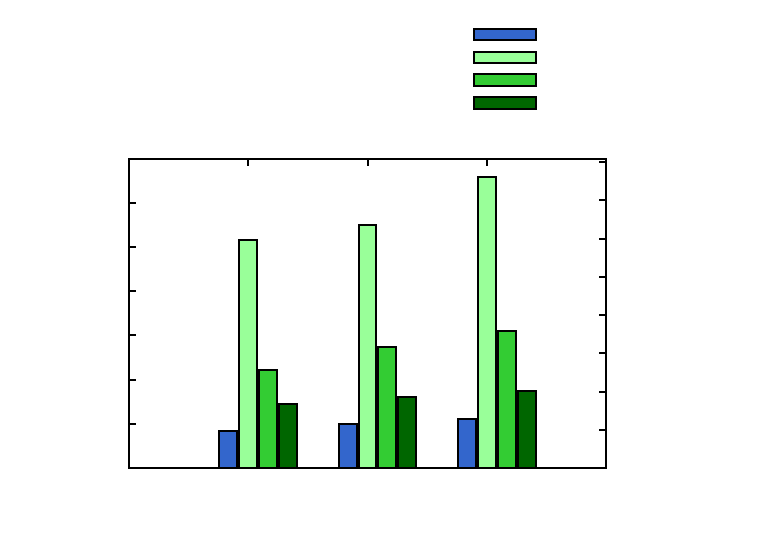
\includegraphics{2_5_sym_all}}%
    \gplfronttext
  \end{picture}%
\endgroup
}
%%   \caption{}
%%   \label{fig:meter_ch_sym_2_5}
%% \end{figure}

%% \begin{figure}[!hb]
%%   \centering
%%   \resizebox{\columnwidth}{!}{% GNUPLOT: LaTeX picture with Postscript
\begingroup
  \makeatletter
  \providecommand\color[2][]{%
    \GenericError{(gnuplot) \space\space\space\@spaces}{%
      Package color not loaded in conjunction with
      terminal option `colourtext'%
    }{See the gnuplot documentation for explanation.%
    }{Either use 'blacktext' in gnuplot or load the package
      color.sty in LaTeX.}%
    \renewcommand\color[2][]{}%
  }%
  \providecommand\includegraphics[2][]{%
    \GenericError{(gnuplot) \space\space\space\@spaces}{%
      Package graphicx or graphics not loaded%
    }{See the gnuplot documentation for explanation.%
    }{The gnuplot epslatex terminal needs graphicx.sty or graphics.sty.}%
    \renewcommand\includegraphics[2][]{}%
  }%
  \providecommand\rotatebox[2]{#2}%
  \@ifundefined{ifGPcolor}{%
    \newif\ifGPcolor
    \GPcolortrue
  }{}%
  \@ifundefined{ifGPblacktext}{%
    \newif\ifGPblacktext
    \GPblacktexttrue
  }{}%
  % define a \g@addto@macro without @ in the name:
  \let\gplgaddtomacro\g@addto@macro
  % define empty templates for all commands taking text:
  \gdef\gplbacktext{}%
  \gdef\gplfronttext{}%
  \makeatother
  \ifGPblacktext
    % no textcolor at all
    \def\colorrgb#1{}%
    \def\colorgray#1{}%
  \else
    % gray or color?
    \ifGPcolor
      \def\colorrgb#1{\color[rgb]{#1}}%
      \def\colorgray#1{\color[gray]{#1}}%
      \expandafter\def\csname LTw\endcsname{\color{white}}%
      \expandafter\def\csname LTb\endcsname{\color{black}}%
      \expandafter\def\csname LTa\endcsname{\color{black}}%
      \expandafter\def\csname LT0\endcsname{\color[rgb]{1,0,0}}%
      \expandafter\def\csname LT1\endcsname{\color[rgb]{0,1,0}}%
      \expandafter\def\csname LT2\endcsname{\color[rgb]{0,0,1}}%
      \expandafter\def\csname LT3\endcsname{\color[rgb]{1,0,1}}%
      \expandafter\def\csname LT4\endcsname{\color[rgb]{0,1,1}}%
      \expandafter\def\csname LT5\endcsname{\color[rgb]{1,1,0}}%
      \expandafter\def\csname LT6\endcsname{\color[rgb]{0,0,0}}%
      \expandafter\def\csname LT7\endcsname{\color[rgb]{1,0.3,0}}%
      \expandafter\def\csname LT8\endcsname{\color[rgb]{0.5,0.5,0.5}}%
    \else
      % gray
      \def\colorrgb#1{\color{black}}%
      \def\colorgray#1{\color[gray]{#1}}%
      \expandafter\def\csname LTw\endcsname{\color{white}}%
      \expandafter\def\csname LTb\endcsname{\color{black}}%
      \expandafter\def\csname LTa\endcsname{\color{black}}%
      \expandafter\def\csname LT0\endcsname{\color{black}}%
      \expandafter\def\csname LT1\endcsname{\color{black}}%
      \expandafter\def\csname LT2\endcsname{\color{black}}%
      \expandafter\def\csname LT3\endcsname{\color{black}}%
      \expandafter\def\csname LT4\endcsname{\color{black}}%
      \expandafter\def\csname LT5\endcsname{\color{black}}%
      \expandafter\def\csname LT6\endcsname{\color{black}}%
      \expandafter\def\csname LT7\endcsname{\color{black}}%
      \expandafter\def\csname LT8\endcsname{\color{black}}%
    \fi
  \fi
  \setlength{\unitlength}{0.0500bp}%
  \begin{picture}(7200.00,5040.00)%
    \gplgaddtomacro\gplbacktext{%
      \csname LTb\endcsname%
      \put(946,704){\makebox(0,0)[r]{\strut{} 0}}%
      \put(946,1059){\makebox(0,0)[r]{\strut{} 50}}%
      \put(946,1413){\makebox(0,0)[r]{\strut{} 100}}%
      \put(946,1768){\makebox(0,0)[r]{\strut{} 150}}%
      \put(946,2122){\makebox(0,0)[r]{\strut{} 200}}%
      \put(946,2477){\makebox(0,0)[r]{\strut{} 250}}%
      \put(946,2831){\makebox(0,0)[r]{\strut{} 300}}%
      \put(946,3186){\makebox(0,0)[r]{\strut{} 350}}%
      \put(946,3540){\makebox(0,0)[r]{\strut{} 400}}%
      \put(946,3895){\makebox(0,0)[r]{\strut{} 450}}%
      \put(2256,484){\makebox(0,0){\strut{}1}}%
      \put(3435,484){\makebox(0,0){\strut{}8}}%
      \put(4613,484){\makebox(0,0){\strut{}14}}%
      \put(5923,704){\makebox(0,0)[l]{\strut{} 0}}%
      \put(5923,1317){\makebox(0,0)[l]{\strut{} 0.1}}%
      \put(5923,1930){\makebox(0,0)[l]{\strut{} 0.2}}%
      \put(5923,2543){\makebox(0,0)[l]{\strut{} 0.3}}%
      \put(5923,3156){\makebox(0,0)[l]{\strut{} 0.4}}%
      \put(5923,3769){\makebox(0,0)[l]{\strut{} 0.5}}%
      \put(176,2299){\rotatebox{-270}{\makebox(0,0){\strut{}$\mathrm{L}_{\mathrm{com}} \; (\,\tau\,)$}}}%
      \put(6692,2299){\rotatebox{-270}{\makebox(0,0){\strut{}$\mathrm{L}_{\mathrm{com}} \; (\,\mu\mathrm{sec}\,)$}}}%
      \put(3434,154){\makebox(0,0){\strut{}number of hops}}%
    }%
    \gplgaddtomacro\gplfronttext{%
      \csname LTb\endcsname%
      \put(4129,4867){\makebox(0,0)[r]{\strut{}\texttt{ch\_asymin\_udn}}}%
      \csname LTb\endcsname%
      \put(4129,4647){\makebox(0,0)[r]{\strut{}\texttt{ch\_asymin\_sm\_all}}}%
      \csname LTb\endcsname%
      \put(4129,4427){\makebox(0,0)[r]{\strut{}\texttt{ch\_asymin\_sm}}}%
    }%
    \gplbacktext
    \put(0,0){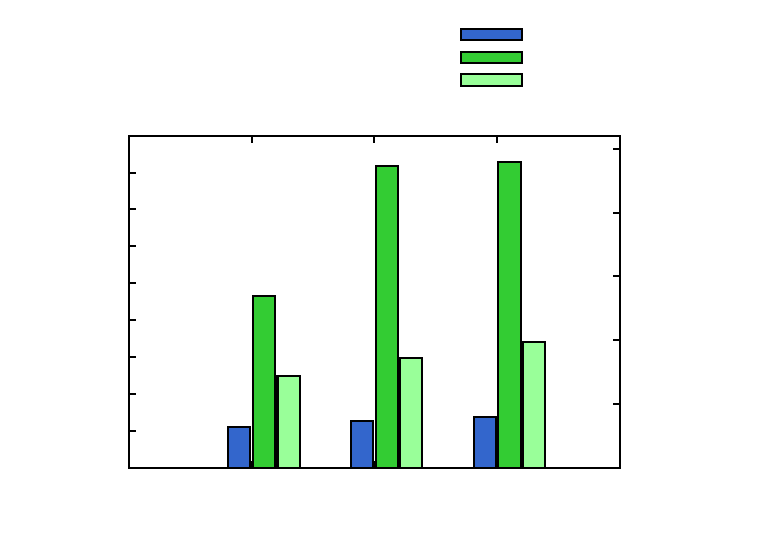
\includegraphics{2_5_asymin_all}}%
    \gplfronttext
  \end{picture}%
\endgroup
}
%%   \caption{}
%%   \label{fig:meter_ch_asymin_2_5}
%% \end{figure}


%%%%%%%%%%%%%%%%%%%%%%%%%%%%%%%%%%%%%%%%%%%%%%%%%%%%%%%%%%%%%%%%%%%%%%%%%%%%%%%%


  
\FloatBarrier


%% \begin{table}[!h]
%%   \centering
%%   \begin{tabular}{|l|l|l|l|l|}
%%     \hline
%%     \multirow{2}{22ex}{\emph{Implemenatation}} & \multirow{2}{*}{\emph{\#Hops}} & \multicolumn{3}{|c|}{$\inLcom \; (\tau)$} \\
%%     \cline{3-5}
%%     & & \emph{Avg} & \emph{Std Dev} & \emph{Max} \\
%%     \hline
%%     \multirow{3}{18ex}{\texttt{ch\_asymin\_udn}} & \\
%%     & \\
%%     & \\
%%     \hline
%%     \multirow{3}{18ex}{\texttt{ch\_asymin\_sm\_no}} & \\
%%     & \\
%%     & \\
%%     \hline
%%     \multirow{3}{18ex}{\texttt{ch\_asymin\_sm}} & \\
%%     & \\
%%     & \\
%%     \hline
%%   \end{tabular}
%%   \caption{Risultati numerici, in cicli di clock, della misurazione della latenza di comunicazione asimmetrica in ingresso delle diverse implementazioni.}
%% \end{table}



%% \begin{table}[!h]
%%   \centering
%%   \begin{subtable}[b]{\textwidth}
%%     \begin{tabular}{|l|l|l|l|l|}
%%       \hline
%%       \multirow{2}{22ex}{\emph{Implemenatation}} & \multirow{2}{*}{\emph{\#Hops}} & \multicolumn{3}{|c|}{$\inLcom \; (\tau)$} \\
%%       \cline{3-5}
%%       & & \emph{Avg} & \emph{Std Dev} & \emph{Max} \\
%%       \hline
%%       \multirow{3}{18ex}{\texttt{ch\_sym\_udn}} & 1 & 42.066550 & 0.097822 & 42.262000 \\
%%       & 8 & 49.561120 & 0.104196 & 49.769500 \\
%%       & 14 & 55.722760 & 0.107943 & 55.792050 \\
%%       \hline
%%       \multirow{3}{18ex}{\texttt{ch\_sym\_sm\_no}} & 1 & 257.800490 & 0.008955 & 257.815900 \\
%%       & 8 & 275.320380 & 0.006685 & 275.327650 \\
%%       & 14 & 329.332180 & 0.018220 & 329.363400 \\
%%       \hline
%%       \multirow{3}{18ex}{\texttt{ch\_sym\_sm}} & 1 & 111.482450 & 0.187050 & 111.653200 \\
%%       & 8 & 137.378440 & 0.016294 & 137.395550 \\
%%       & 14 & 155.377520 & 0.013281 & 155.393950 \\
%%       \hline
%%       \multirow{3}{18ex}{\texttt{ch\_sym\_sm\_nullack}} & 1 & 72.359500 & 0.219423 & 72.549500 \\ 
%%       & 8 & 80.700840 & 0.124463 & 80.827350 \\ 
%%       & 14 & 86.759230 & 0.118203 & 86.826250 \\
%%       \hline
%%     \end{tabular}
%%     \caption{Misurazione della latenza di comunicazione simmetrica delle diverse implementazioni.}
%%   \end{subtable}

%%   %%%%%%%%%%%%%%%%%%%%%%%%%%%%%%%%%%%%%%%%%%%%%%%%%%%%%%%%%%%%%%%%%%%%%%%%%%%%%%%%
%%   \vspace{4ex}
%%   %%%%%%%%%%%%%%%%%%%%%%%%%%%%%%%%%%%%%%%%%%%%%%%%%%%%%%%%%%%%%%%%%%%%%%%%%%%%%%%%

%%   \begin{subtable}[b]{\textwidth}
%%     \centering
%%     \begin{tabular}{|l|l|l|l|l|}
%%       \hline
%%       \multirow{2}{22ex}{\emph{Implemenatation}} & \multirow{2}{*}{\emph{\#Hops}} & \multicolumn{3}{|c|}{$\inLcom \; (\tau)$} \\
%%       \cline{3-5}
%%       & & \emph{Avg} & \emph{Std Dev} & \emph{Max} \\
%%       \hline
%%       \multirow{3}{18ex}{\texttt{ch\_asymin\_udn}} & 1 & 56.025529 & 0.000941 & 56.026905 \\
%%       & 8 & 63.525349 & 0.000979 & 63.526575 \\
%%       & 14 & 69.527121 & 0.001011 & 69.528720 \\
%%       \hline
%%       \multirow{3}{18ex}{\texttt{ch\_asymin\_sm\_all}} & 1 & 230.570268 & 0.028743 & 230.643940 \\
%%       & 8 & 408.779285 & 0.047859 & 408.846645 \\
%%       & 14 & 414.374837 & 0.025326 & 414.417200 \\
%%       \hline
%%       \multirow{3}{18ex}{\texttt{ch\_asymin\_sm}} & 1 & 125.039207 & 0.001632 & 125.041220 \\
%%       & 8 & 149.041103 & 0.001936 & 149.045050 \\
%%       & 14 & 170.037299 & 0.002036 & 170.040285 \\
%%       \hline
%%     \end{tabular}
%%     \caption{Misurazione della latenza di comunicazione asimmetrica in ingresso delle diverse implementazioni.}
%%   \end{subtable}

%%   \caption{Misure della latenza di comunicazione rilevate iterando 10 volte il programma ``ping-pong'' con $m = 10^5$ scambi }

%% \end{table}


